\chapter{Introduction}
\label{c:intro}

\section{Motivation}

\begin{figure}[htb]
  \centering
  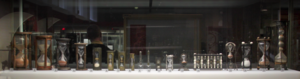
\includegraphics[width=1.0\columnwidth]{hour_glasses.png}
  \caption{Hour glasses at the London Science Museum.}
\label{fig:hour_glasses} 
\end{figure}

\graphicspath{{10-introduction/images/}}

\greybox{We may ask ourselves how we would create a single model that could create all of the hour glasses in Figure~\ref{fig:hour_glasses}. This is the goal in \emph{procedural geometric modeling} -- we have no definitive way to do this today, but in this document we hope to take some steps towards a solution.

Whilst a standard 3D work flow might allow a user to create a single hour glass of a specific dimension and design, a procedural modeling system might let a user create an algorithm that produces a glass of any given dimension. 
}

Procedural geometric modeling (\emph{PGM}) is a field studying algorithms that compute geometry. A procedural model consists of a sequence of parametrised operations that are able to automatically construct a variety of geometric forms. 

The additional level of abstraction offered by PGM has significant benefits over single-instance modeling, but introduces a number of challenges. The advantages of PGM include:

\begin{itemize}
\item{An arbitrary quantity of geometry can be created to describe a virtual environment in constant time; the time it takes to construct the procedural model.}
\item{The removal of the existing restriction that the size of a virtual environment is proportional to the time spent creating it.}
\item{The quality of the environment is consistent at no additional cost.}
\item{Procedural geometry tools could lead to run­time environment generation. A virtual world can be generated as the user explores it, giving an experience with more variety and less repetition to the user~\cite{Hahn06}}. 
\item{Procedural methods offers the potential to generate content that reacts to various stimuli. For example it could respond to current hardware availability, to users' level of expertise, the length of their attention span, or the medium on which it is presented.}
\end{itemize}

One particular application that has become a testbed for the concepts of PGM is urban modeling. In 2010, half of the people in the world lived in cities, and this fraction is increasing. Cities form the backdrops to large portions of our lives; the way they are designed, how they look, how we think about them, and how we get around them directly affects us all. With the rise of computer graphics, creating cityscapes in virtual worlds has become a common task in a wide range of disciplines such as architecture, city planning, 3D cartography, video games and cinema. 

However, creating virtual representations of cityscapes is expensive. At the crudest level, paying an artist to attach a door-handle to every door in every building in a town is costly. Alternately we may obtain 3D city geometry by reconstructing photographs, but obtaining the photos is difficult, and the results often have a lot of noise. Furthermore, the cities that we wish to model may not yet exist, may have only existed before the invention of photography, or be entirely fictional. PGM offers a solution to these issues by promising to generate large quantities of characteristic geometry very quickly. The real world applications of urban procedural modeling are growing, recent examples include ---

\begin{itemize}
\item{Masdar is a new city, designed and built entirely on undeveloped land outside Abu Dhabi. The initial project is intended to be completed in 2015 and will cover $10^6 m^2$\cite{masdarCity2}. Given the large quantity of architecture that had to created, one of the designers turned to PGM, in the form of CityEngine\cite{cityEngine} to design the Swiss Quarter of the city\cite{masdarCity}.}

\item{Video games can use procedural technology to create new locations as the player explores. For example Dwarf Fortress~\cite{dwarfFortress} generates the terrain, structures and inhabitants of a virtual world procedurally. In this situation the key advantage is that a player may continually explore and discover unique structures, that neither they, nor anyone else, have seen before. }

\item{When the first \emph{Superman} movie was filmed in 1978 computer graphics were in their infancy. To give the appearance of Superman flying, Christopher Reeve was composited on top of footage from New York City, as a stand in for the fictional city of Metropolis. In contrast the 2013 release of \emph{Man of Steel} portrayed the same fictional city, this time generated using the PGM tools Houdini\cite{houdini} and CityEngine\cite{EffectsOmelette}. The advantages of PGM in this situation is that an entirely unrecognisable yet realistic fictional city could be created. Additionally, because the model was digital it could be realistically destroyed by a physical simulation of the alien invaders.}

\end{itemize}

%% discuss some approaches to PGM, and the problems that are encountered. then list specifically.

Given the promise of PGM, it makes sense to question why it isn't the standard technique for geometry creation. Designing procedural models is more complex; the designer must not just design a single item of geometry, but a continuum. Current state-of-the-art systems rely extensively on programming paradigms for users to construct useful and powerful procedural models. In summary, the drawbacks of current PGM include ---

\begin{itemize}
\item{Designers must undertake the more complex task of designing a class of geometry, rather than a single instance.}
\item{Traditional artists are not familiar with classical methods of describing algorithms, such as programming languages.}
\item{Traditional software engineers do not possess a classically trained sense of aesthetic.}
\item{There are a large number of use cases of PGM, with each likely to require different solutions. 
%We explore some of these in Chapter~\ref{c:readings}.
} 
\end{itemize}

In this thesis we are concerned with removing several of these drawbacks, specifically the requirement that current PGM systems require considerable programming expertise.

\section{Hypothesis}
\label{c:intro:thesisstatement}

We propose that a geometric construct, the \emph{straight skeleton}, and its generalisations, are a powerful technique for the creation of PGM systems that are accessible to people without programming skills.  Systems exploiting these skeletons and variations thereof are able to generate large scale, varied and highly realistic results within the domain of urban procedural modeling.

\section{Contributions}

Our contributions to the corpus while examining the above hypothesis include:

\begin{itemize}
\item{A simplification of existing straight skeleton events, the \emph{generalised intersection event}.}
\item{A novel skeleton, the \emph{mixed weighted straight skeleton}.}
\item{A method and evaluation of a system for procedural modeling of city lot shapes using the straight skeleton.}
\item{A method and evaluation for the procedural modeling of architectural shells using the MWSS.}
\end{itemize}

The papers written in the course of this thesis were:
\begin{itemize}

\item{\emph{Interactive Architectural Modeling with Procedural Extrusions}\cite{twak11}}
\item{\emph{Procedural Generation of Parcels in Urban Modeling}\cite{twak12}}

\end{itemize}


%==============================================================================


\section{Overview}

To lay the ground for this work Chapter 2 examines existing work, and describes the properties of existing procedural systems. We continue to analyse the straight skeleton in Chapter 3 and to apply the skeleton to the problem of urban procedural modeling in Chapters 4 and 5. 

The following chapter samples the wide range of tools available for the generation of 3D geometry. In particular we observe that an offset mechanism driven by the straight skeleton is a powerful accompaniment to a written programming language. This insight lead us to examine skeletons in greater detail.

\begin{figure*}
  \centering
  \def\svgwidth{0.7\columnwidth}
  \includesvg{12-skeleton/images/skel_shrink}
  \caption[Shrinking a polygon to form the straight skeleton]{\label{fig:skel_shrinkINTRO}Left: A shrinking polygon. Right: The arcs of the straight skeleton (blue) are formed by tracing the edges of the shrinking polygon.}
\end{figure*}

The straight skeleton is a geometric construct that subdivides a 2D shape, as introduced in Fig.~\ref{fig:skel_shrinkINTRO}. In Chapter 3 we analyse this construct and develop the theory behind the types of degeneracy encountered when computing the straight skeleton. By relaxing the constraints on this structure we introduce a novel variation, the mixed weighted straight skeleton. In addition we introduce a simplification of existing skeleton events, the generalised intersection event. These skeletons have interesting non-trivial properties, such as being able to split concave shapes into two, introducing holes into faces, and leaving behind ``arcs'' which form part of the centrelines of a shape. It is these emergent properties that we found we could exploit to create an expressive range of procedural geometry. 

\begin{figure*}
\centering
\def\svgwidth{1.0\columnwidth}
\includesvg{14-parcels/images/cityengine}
\caption[CityEngine results]{\label{fig:cityEngineINTRO}The results of our parcel subdivision algorithm within CityEngine. Left: The parcel subdivision generated with both skeleton (bottom left of grey line) and OBB (top right) techniques; the colouring denotes relative area. Right: the result of the urban procedural modeling pipeline within CityEngine.}
\end{figure*}

The first application of these properties is to the problem of subdividing city blocks to many parcels of land. We introduce the first complete algorithms and evaluation of block subdivision within computer graphics. In addition, we demonstrate how subdivision can take place without additional end user programming by presenting a parameterised algorithm that utilises the straight skeleton, as illustrated in Fig.~\ref{fig:cityEngineINTRO}. The results of this system are presented at the end of Chapter 4, and evaluated favourably again real-world subdivisions and existing block subdivision schemes.


\begin{figure*}
  \centering
  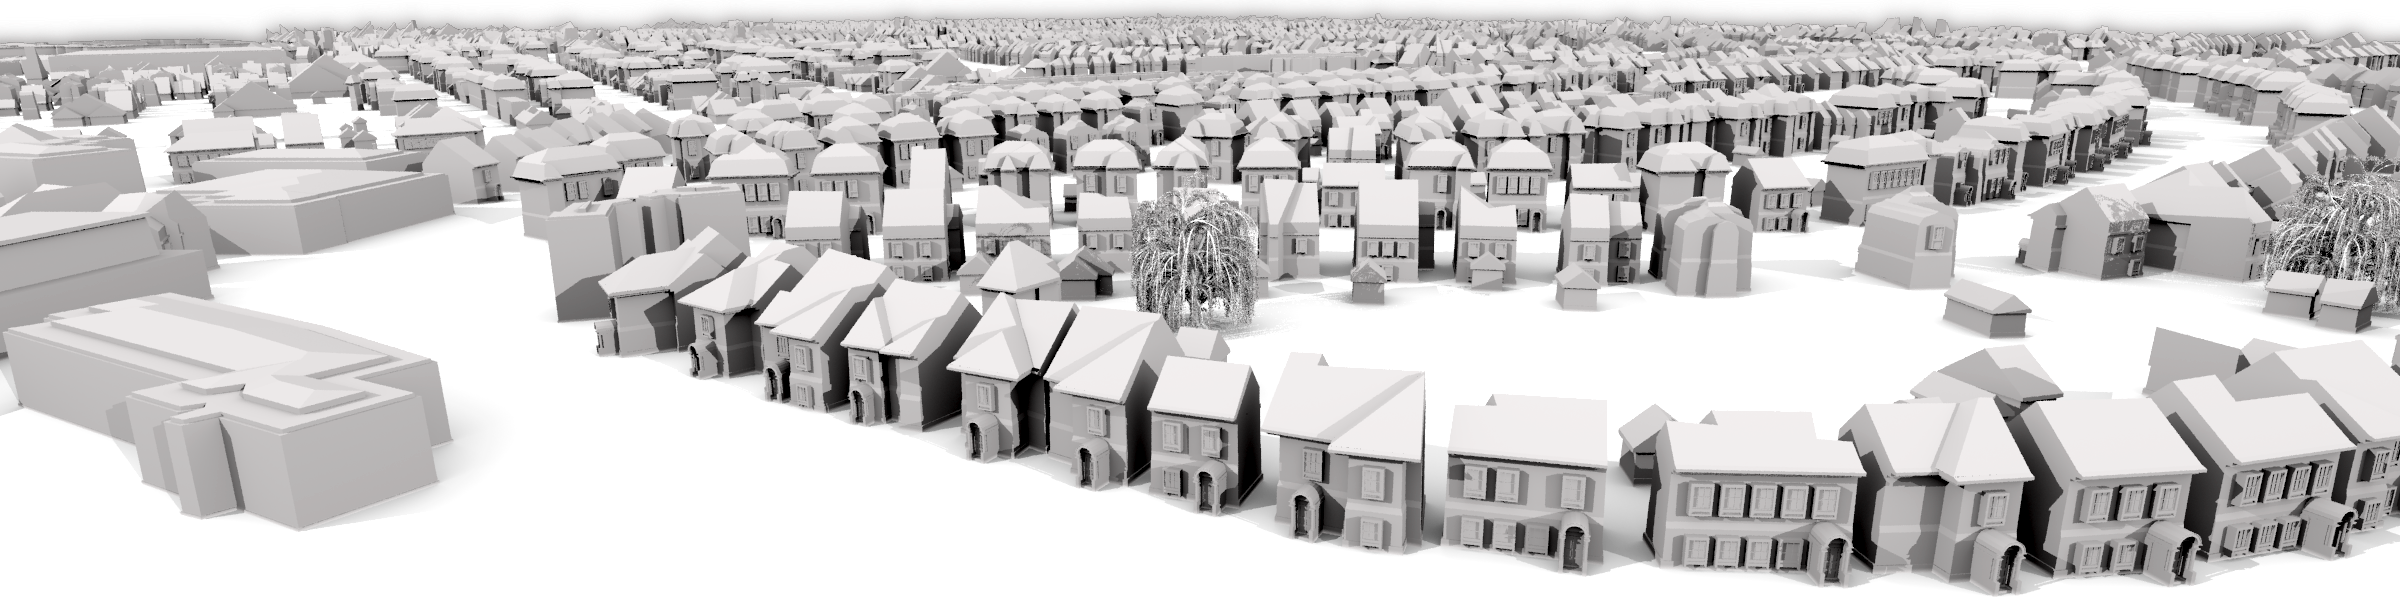
\includegraphics[width=1.0\columnwidth]{strip.png}
  \caption[Large scale GIS results]{\label{fig:StripINTRO} We present an interactive procedural modeling system that is able to model difficult architectural surfaces, such as roof constructions. This figure shows procedural extrusions applied to 6000 floorplans  synthesised from a GIS database of Atlanta. Procedural trees were added for decoration.}
\label{fig:teaser}
\end{figure*}


The second application is the creation of solid architectural models. By using a novel generalisation of the straight skeleton, Chapter 5 demonstrates how to create complex architectural models, containing features such as buttresses, chimneys, bay windows, columns, pilasters, and alcoves. We introduce two user interfaces, one for the interactive specification of such geometry, and another for the procedural generation architectural models from floorplans over wide areas, as shown in Fig.~\ref{fig:StripINTRO}. The system is evaluated both for its expressiveness, by modeling a wide range of existing architecture, and robustness, by automatically generating a large cityscape.

We conclude in Chapter 6, arguing that procedural geometric modeling without written programming languages is possible using the straight skeleton. Systems exploiting these skeletons and variations thereof are able to generate large scale, varied, and highly realistic results within the domain of urban procedural modeling.

\begin{comment}
\newpage

\section{Corrections checklist}
\label{sec_corrections}

Edited body text has been highlit in \twak blue\kawt, but this doesn't work in captions or for images. The following corrections have been made:

\begin{itemize}
\item{Add more detail to the abstract.}
\item{This corrections section, Sec.\ref{sec_corrections}}
\item{Document title to include ``straight skeleton''}

\item{ch1 motivate city creation in chapter 1, turn it into more of a story}

\item{Sec. 1.2 relabel as \emph{hypothesis}, and spell out contributions, giving forward refs to the other chapters. A thumbnail sketch. For each chapter, add more context, why this direction was chosen}

\item{End of chapter 2 ; a comment on the state of the art, what can skeletons do?. What is lacking, why skeletons can make a contribution: Sec.~\ref{s:readingsSummary}}

\item{Missing an approach section. given state of the art from chapter 2, what methods will I use to tackle the problem. Sec.~\ref{s:approachingTheMiddle}}

\item{Chapter 3: Sec.\ref{sec_ways_of_shrinking} bullet points starts with b}

\item{ for each of chapters $\in \{4,5\}$:}
\begin{itemize}
\item{add additional context at start} 
\item{conclusion: clearly state contribution in conclusions (bullet points if necessary)}
\item{conclusion: summarise process and results more verbosely}
\end{itemize}
\item{Brief discussion of the nature of evaluating procedural content, sub Sec.~\ref{sec:evalParcels}}
\item{Justify metrics in the introduction to the chapter, Sec.~\ref{sec:evalParcels}}

\item{Chapter 4: illustrate and justify why we couldn’t have used the medial axis approximations? - Sec.~\ref{sec:skeletonSubivision}}
\item{diagram illustrating medial axis issues in parcel media section: Fig:\ref{fig:medialIssues}}
\item{Remove bits from ch4 which were not my work - the \textdagger stuff; Sec.\ref{sec:parcelIOandGoals}, \ref{sec:parcelIntroduction} and the introductory grey box had referring material removed.}
\item{make sure pictures and text appear in correct order: ensured all text came before all images in Chapter 4}

\item{Chapter 5: Add a URL for siteplan (the procedural extrusion implementation) in Sec.~\ref{sec:UI:overview}}


\item {Discuss \& justify not creating roofs with the medial axis; an example medial axis roof (approx using polygons) Fig.\ref{fig:vsmedial} in Sec.~\ref{sec:alternatives}}


\item{A similar figure as on page 52 to demonstrate the quality of existing meshes (untextured, rendered in same way) ~\ref{fig:googleWarehouseComp}, referenced in body of Secs.~\ref{Sec:Results} and ~\ref{sec:alternatives}. Descriptions of typical the typical construction process in Fig. \ref{fig:mesh} are referenced.}

\item{state that all 50 building examples were successfully modelled, Sec.~\ref{Sec:Results}}

\item{Example of editing a profile, which causes the roof to change phase. Discussion of non-smooth regions in parameter space (borderline cases), and how they affect the users. Fig.~\ref{fig:discontinuities} in Sec.~\ref{Sec:Results}.}

\item {Clarify what happened in the 50 model creation, and the variation in the modelling times: why so long to to create? how many edits, how many trials required? In Sec.~\ref{s:the_modeling_process}.}

\item {Typos from printed manuscripts (mostly not \twak coloured \kawt)}


\item{conclusions too light: Expanded Sec.\ref{c:conclusion}. bulk it out a bit. Be formulaic. (as in notes).}

\item{spell check - not highlighted in blue}

\end{itemize}

\end{comment}
